% \documentclass[acmsmall]{acmart}
\documentclass[sigconf]{acmart}
\usepackage[UTF8, fontset=macnew]{ctex}
\usepackage{graphicx}
\graphicspath{ {./images/} }


%%
%% \BibTeX command to typeset BibTeX logo in the docs


%%
%% Submission ID.
%% Use this when submitting an article to a sponsored event. You'll
%% receive a unique submission ID from the organizers
%% of the event, and this ID should be used as the parameter to this command.
%%\acmSubmissionID{123-A56-BU3}

%%
%% The majority of ACM publications use numbered citations and
%% references.  The command \citestyle{authoryear} switches to the
%% "author year" style.
%%
%% If you are preparing content for an event
%% sponsored by ACM SIGGRAPH, you must use the "author year" style of
%% citations and references.
%% Uncommenting
%% the next command will enable that style.
%%\citestyle{acmauthoryear}

%%
%% end of the preamble, start of the body of the document source.
\begin{document}

%%
%% The "title" command has an optional parameter,
%% allowing the author to define a "short title" to be used in page headers.
% \title{Learn How to write a apporpriate resume by example - The preliminary text mining on the open data}
% \title{透過實際案例學習如何撰寫好的求職履歷 - 使用文字探勘技術之初步研究}
\title{求職履歷探勘 - 非監督式跨領域履歷辨認與視覺化}

%%
%% The "author" command and its associated commands are used to define
%% the authors and their affiliations.
%% Of note is the shared affiliation of the first two authors, and the
%% "authornote" and "authornotemark" commands
%% used to denote shared contribution to the research.

\author{李昀潔}
\affiliation{%
    \institution{資管博一}
}
\author{呂孟芸}
\affiliation{%
    \institution{國企四}
}
\author{張譯心}
\affiliation{%
    \institution{國企四}
}
\author{陳韋霖}
\affiliation{%
    \institution{資工碩一}
}
\author{詹雅安}
\affiliation{%
    \institution{會計四}
}

%%
%% By default, the full list of authors will be used in the page
%% headers. Often, this list is too long, and will overlap
%% other information printed in the page headers. This command allows
%% the author to define a more concise list
%% of authors' names for this purpose.
% \renewcommand{\shortauthors}{Trovato and Tobin, et al.}

%%
%% The abstract is a short summary of the work to be presented in the
%% article.
\begin{abstract}
    對於學生而言,除了努力完成學業或完成研究以取得畢業之外,
    如何透過簡歷(Resume)的撰寫去應徵企業的招募也是一件重要的事,
    另一方面對於欲招聘員工之企業而言,
    如何在海量的履歷中,有效率找到合適之員工也是一件值得關注的議題。
    因此本專案從網際網路上找尋到個人履歷之開放資料集,
    並以此資料提出一簡易之文字探勘方式,
    來回應上述兩個問題。

    本專案共提出了兩種方法,
    其一為檢驗履歷的寫法是否能對應到公司招聘的職位,
    透過文字分群方法(Clustering)來看出該些資料是否與其由請之職位是否相符,
    其二為找出跨領域之人材,
    透過一簡易算式,使得公司能夠有效率地找出具有跨領域特性之申請者,
    進而減少人力去人工檢視履歷之成本。
    此次研究希望透過該開放資料集所作的初步研究,
    希望能對學生們製作個人簡歷上能有所幫助,
    也希望此提出之簡易方法能幫助讀者面臨篩選履歷之問題。
\end{abstract}

%%
%% The code below is generated by the tool at http://dl.acm.org/ccs.cfm.
%% Please copy and paste the code instead of the example below.
%%

\begin{CCSXML}
<ccs2012>
   <concept>
       <concept_id>10010405</concept_id>
       <concept_desc>Applied computing</concept_desc>
       <concept_significance>500</concept_significance>
       </concept>
   <concept>
       <concept_id>10010405.10010497</concept_id>
       <concept_desc>Applied computing~Document management and text processing</concept_desc>
       <concept_significance>500</concept_significance>
       </concept>
 </ccs2012>
\end{CCSXML}

\ccsdesc[500]{Applied computing}
\ccsdesc[500]{Applied computing~Document management and text processing}

\ccsdesc[500]{Applied computing}


%%
%% Keywords. The author(s) should pick words that accurately describe
%% the work being presented. Separate the keywords with commas.
% \keywords{datasets, neural networks, gaze detection, text tagging}

%% A "teaser" image appears between the author and affiliation
%% information and the body of the document, and typically spans the
%% page.
\iffalse
\begin{teaserfigure}
  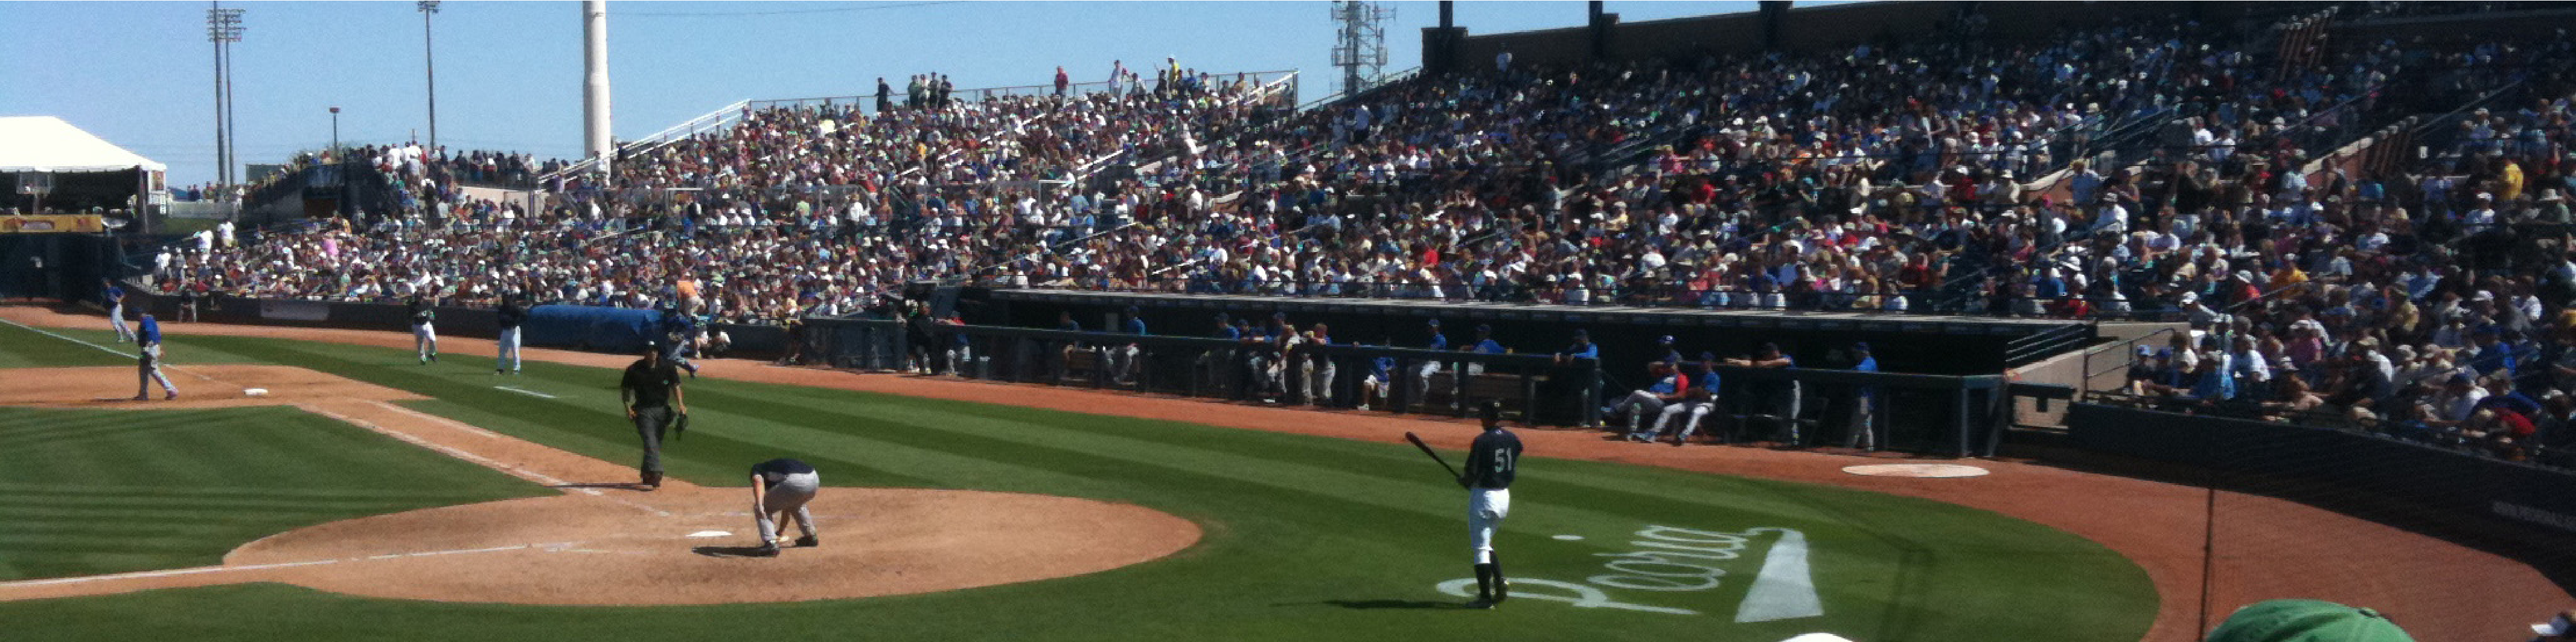
\includegraphics[width=\textwidth]{sampleteaser}
  \caption{Seattle Mariners at Spring Training, 2010.}
  \Description{Enjoying the baseball game from the third-base
  seats. Ichiro Suzuki preparing to bat.}
  \label{fig:teaser}
\end{teaserfigure}
\fi

%%
%% This command processes the author and affiliation and title
%% information and builds the first part of the formatted document.
\maketitle

\section{研究目標}

投履歷找工作時,
如何撰寫一份符合業主要求的履歷,
尤其對於高度專業的工作而言,
更顯重要,
然如何撰寫履歷等事宜,
雖坊間有許多教條方法供大眾學習,
但寫法上需考慮求職者的狀況,
並無法直接使用法則來套用。
有鑑於此,
我們使用網路上公開之求職簡歷資料,
運用課堂所學習之文字探勘技術來針對該些資料進行分析,
藉此探求有趣的訊息以幫助求職者來面對如何撰寫履歷之問題。

另一方面,
對於企業主而言,
如何在大量之履歷文件中,
有效率找到合適之人員,
也是一門重要的課題,
而履歷為文本資料,
難以透過簡單之公式運算,
諸如單一以學歷或年資來篩選,
都有可能因此剔除掉適合之人員,
且求職者之專業能力,
皆呈現於文字之表達,
不易透過單純之量化分析來取得此資訊,
因此我們針對此問題,
希望提出一簡易之文字探勘方法,
來幫助企業主能夠在面對大量求職者履歷中,
透過該些履歷資料內容,
使用履歷內含之資料自動分析出結果,
使其能有效率地找出合適之履歷。

於本專案中,
我們設定了兩個主題進行探討,
其一為驗測該些資料是否各對應之履歷內容是否符合該求職之工作,
其二為找出部份具有跨領域特性之履歷。

\section{方法}

本專案中,
我們所探討之資料,
為從網路上所抓下來之公開資料,
而該些資料除了各履歷的內容外,
也包含了各別履歷所對應之求職職位。

以文字探勘而言,
雖然求職職位與其履歷資料這兩種資料型可視為一種監督式學習技術之應用(Supervised Learning)\cite{murphy2012machine}。
然於本專案中,
欲探討之主體非以分類問題之面象而進行之,
而是希望從資料本身特性出發,
藉由資料分析方法,
試圖找出有趣的履歷範本,
意即透過非監督式學習技術(Unsupervised Learning)\cite{murphy2012machine}。

關於內容,
共分為兩項方法,
第一我們提出如何檢驗資料內容是否一致,
意即我們想確認是否各求職類別是否對應該些求職履歷,
透過分群的方法去檢驗是否各群集(Cluster)內是否有內聚,
第二透過資料本身性質找出具跨領域性質之履歷,
並順便將找尋之結果作為範本供讀者參考,
其方法上我們視此該些資料視為資料探勘問題\cite{han2011data},
以找出適合之履歷資料。

\subsection{資料集}

針對履歷資料,
我使用了公開資料集作為本專案之資料,
其以Kaggle網站公開之實際之工作求職者履歷資料進行分析\cite{kaggle_dataset},
該資料共擁有三個欄位,
分別為ID,
Resume\_str,
Resume\_html及Category,
ID欄位表示流水號,
中間兩欄位分別為Resume的純文字及其原始抓下來的格式(內含HTML標籤),
Category表示對應所求職之職位名,
此資料集共有24個求職職位,
求職種類及數量表可參照圖.~\ref{counter_of_application}。
資料集共有2484筆資料(resumes)。

\begin{figure}
    \centerline{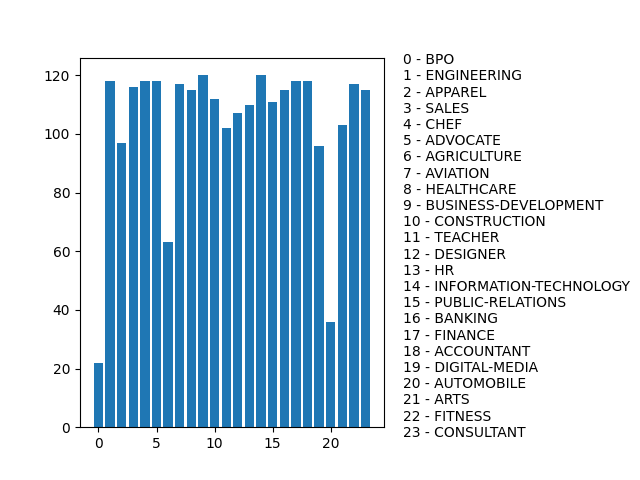
\includegraphics[width=0.5\textwidth]{counter_of_application.png}}
    \caption{The counting for each application catogery in the resumes}
    \label{counter_of_application}
\end{figure}

\subsection{資料前處理}

於本專案中,
我們主要進行兩項工作,
然而在進行之前,
我們需要進行資料前處理工作,
才能將履歷資料轉換成我們可以分析的資料,
在開始分析前,
我們會將履歷中各個多餘空格去除,
避免該些空格造成分析上的偏誤。

我們透過使用Sentence-Transformers\cite{reimers-2020-multilingual-sentence-bert}工具,
將資料集之真實履歷資料,
透過BERT方法\cite{devlin2018bert},
將該些履歷內的文字,
轉成合適之word embeddings。
該些word embeddings為資料集中,
所有履歷之文字,
經過轉換後之新資料表示法,
其原因為,
若不經過轉換,
原始資料中所有文字所表示之方法,
其通常表示法可能為詞袋(bag of word)或是one-hot encoding編碼等,
但這些表示法都有空間浪費的問題,
因為所有文字所產生之矩陣(Matrix)都具有高度稀疏性\cite{schutze2008introduction},
因此提出透過BERT轉換\cite{devlin2018bert},
將原有的矩陣維度進行降維(dimension reduction),
可在保存原有資料的特徵外,
減少了原本高度稀疏所造成的問題。

\subsection{履歷一致性}

在取得word embeddings後,
我們會先針對此資料,
透過python的sklearn\cite{sklearn_api}套件,
使用資料探勘之常見分群方法(k-means clustering)進行檢驗\cite{han2011data},
其目的為自動分析履歷資料之性質是否於其目標求職職缺有相符,
意即針對特定群體之履歷,
其所對應之相同職缺,
該些個別履歷資料之特性應具有相似性,
我們將採用k-means分群方法\cite{macqueen1967some}進行分析。

此目一種簡易之分析法及視覺化方法,
目的為檢驗是否在特定之職缺資料內,
該對應之履歷料有相符。

%第三種分群方法,
%我們採用DBSCAN(Density-based spatial clustering of applications with noise)DBSCAN\cite{ester1996density},

\subsection{具跨領域性質之履歷}

我們希望能找到是否有具跨領域性質之履歷,
因此希望找出該些履歷離所屬之職務類別之核心履歷越遠越好,
且該履歷可能與其他職缺很相近。

因此
為達此目的,
我們共進行三個步驟,
令$D$為所有履歷之集合,
$C$為所有職缺類別之集合,
而$d_{c}$則表示為所於職缺$c$之履歷$d$,
我們計算各職缺類別之平均中心向量如公式 \ref{overline}所示,
之後我們將利用平均中心向量求得各職務群內之核心履歷$\hat{d}$如公式 \ref{d_hat} 所示,
再將該核心履歷 $\hat{d}$拿來求得該職務群內最不相似之履歷 $d^{*}$,如公式 \ref{d_star} 所示,
並將其視為具有跨領域性質之履歷,
其計算相似度之方法,我們使用餘弦相似度計算式(cosine similarity)\cite{schutze2008introduction},
最後我們用$d^{*}$來計算離其最近之職務群如公式 \ref{eq:d_bar} 及公式 \ref{eq:c_dot} 所示,
$D_{c^{'}}$表示為找出之與具有跨領域性質之履歷$d^{*}$相似之求職類別之文件集合。
用以來觀察該履歷$d^{*}$是否具有跨領域之性質。

\begin{equation}
    \label{overline}
    \overline{d}_c := \frac{1}{|d_{c}|}\sum_{i=1}^{|d_{c}|}{d_{c,i}}\;, \quad c\in C, d\in D.
\end{equation}

\begin{equation}
    \label{d_hat}
    \hat{d}_c := \arg \max_{k} sim(\overline{d_{c}}, d_{k \in c}).
\end{equation}

\begin{equation}
    \label{d_star}
    d^{*}_c := \arg \min_{k} sim(\hat{d}_c, d_{k \in c}).
\end{equation}

\begin{equation}
    \label{eq:d_bar}
    \overline{d}_{c^{'}}=\begin{cases}
    \overline{d}_{c^{'}} := \frac{1}{|d_{c^{'}}|}\sum \limits_{}^{|d_{c^{'}}|}{d_{c^{'}}}, & \text{if $|c^{'}| \leq 1$}.\\
    \overline{d}_{c^{'}} := \frac{1}{|c^{'}|} \sum \limits_{}^{|c^{'}|} \frac{1}{|d_{c^{'}}|}\sum \limits_{}^{|d_{c^{'}}|}{d_{c^{'}}}, & \text{otherwise}.
  \end{cases}
\end{equation}

\begin{equation}
    \label{eq:c_dot}
    D_{c^{'}} := \{ d_{c^{'}}  : \arg \min_{c^{'}} sim(d^{*}_{c}, \overline{d}_{c^{'}}) \}
\end{equation}


\section{研究結果}

於本專案中,
我們所使用之實驗機器規格為一般配有GPU之個人電腦,
CPU為AMD Ryzen Threadripper 1920X 12-Core Processor,
其核心數為24,
作業系統版本為Ubuntu 16.04.5 LTS,
記憶體為125G,
GPU為GeForce RTX 2080 Ti。

\subsection{履歷一致性}

\begin{figure}
    \centerline{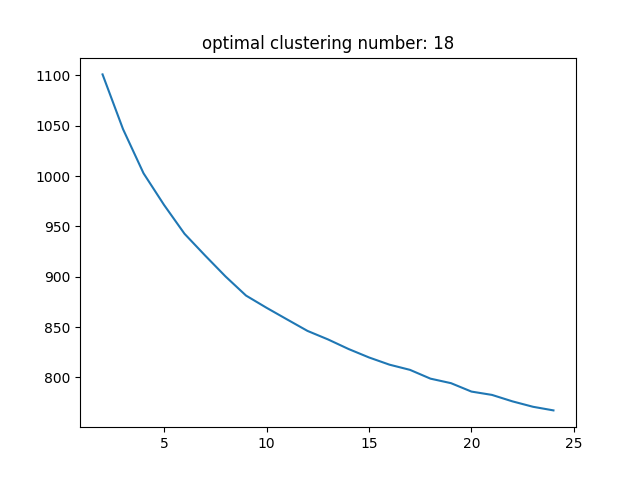
\includegraphics[width=0.5\textwidth]{elbow_method.png}}
    \caption{Elbow method for finding the optimal clustering number}
    \label{elbow_method}
\end{figure}

\begin{figure}
    \centerline{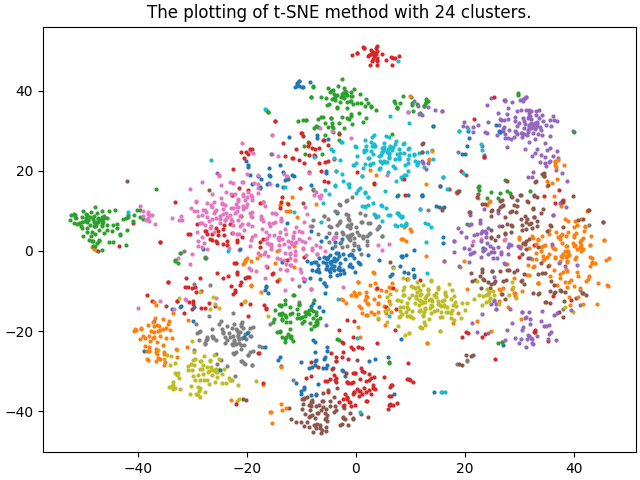
\includegraphics[width=0.5\textwidth]{t_sne.png}}
    \caption{The result of t-SNE for k-means clustering}
    \label{t_sne}
\end{figure}

\begin{figure}
    \centerline{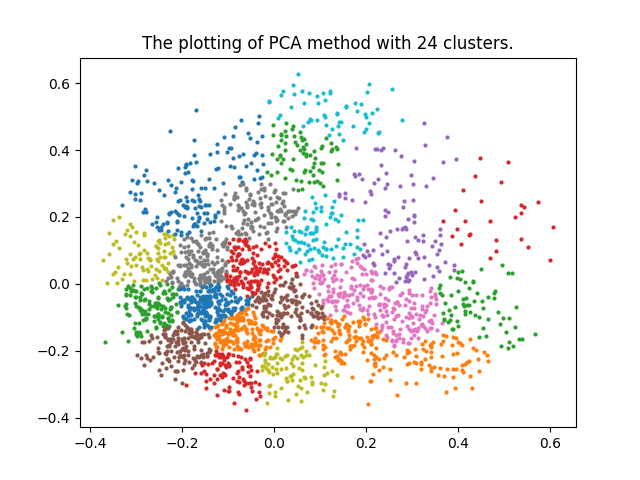
\includegraphics[width=0.5\textwidth]{pca.png}}
    \caption{The result of PCA for k-means clustering}
    \label{pca}
\end{figure}

\begin{figure}
    \centerline{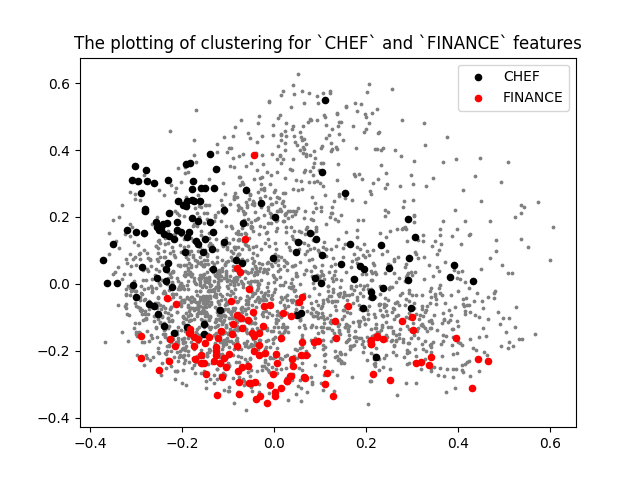
\includegraphics[width=0.5\textwidth]{chef_finance_plotting.png}}
    \caption{The plotting between `CHEF` and `FINANCE` applications}
    \label{chef_finance_plotting}
\end{figure}


為了要檢驗資料中的履歷是否與該申請之職缺相符,
我們使用了k-means\cite{macqueen1967some}作為分群方法,
利用elbow method來取得最適分群數(Optimal clustering number),
其結果如圖.~\ref{elbow_method},
所得值為18,
對照原來之職缺總數共計24項,
可看出差距雖為6,
應不是顯著數字,
從此差距數字下,
我們可推論不同的申請之職業類別的群集結與自動分群結果相似,

另外我們也使用了Adjusted Rand Index來評價分群的結果\cite{hubert1985comparing},
k-means分群結果所得之Adjusted Rand Index為0.192,
其值大於零,
因此具有分群結果具有可信性,
然其值看似不接近於1,
可推論為該些履歷內含有求職者個人化訊息,
加大了資料間的離散程度。

針對結果,
我們採用PCA(Princial Component Analysis)\cite{pearson1901liii} \cite{han2011data}將k-means之分群結果進行降維,
將word embeddings維數降成兩維,
如圖.~\ref{pca}所示,
各顏色代表各別之職缺類別,
而我們也隨機抽樣兩種職缺進行畫圖,
如圖.~\ref{chef_finance_plotting}所示,
由此圖可看出類別間應具一定的差異性。


另一方面,
雖PCA為資料探勘之常見方法,
但因為資料全為文字,
所以我也使用了t-SNE(t-Distributed Stochastic Neighbor Embedding)\cite{van2008visualizing}作為補助判斷 ,
如圖.~\ref{t_sne}所示,
各顏色代表各別之職缺類別,
雖不若PCA結果如此一致,
但仍可看出各類別間的分群結果具有一定差異性。

因此我們可推論,
當要處理一群履歷及其對應之求職職缺之問題時,
此方方法具一定可行性。

\begin{table}[t]
\centering
\resizebox{\columnwidth}{!}{%
\begin{tabular}{|l|l|l|l|l|}
\hline
$c$                 & $c^{'}$                & $\hat{d}$ & $d^{*}$ & similarity  \\ \hline
ACCOUNTANT             & FITNESS                & 21338490   & 24799301    & 0.62522 \\ \hline
ADVOCATE               & HEALTHCARE             & 36392131   & 21614256    & 0.45807 \\ \hline
AGRICULTURE            & DIGITAL-MEDIA          & 19532392   & 34141299    & 0.53679 \\ \hline
APPAREL                & ADVOCATE               & 27176039   & 35121930    & 0.58595 \\ \hline
ARTS                   & ENGINEERING            & 36379931   & 26069113    & 0.33301 \\ \hline
AUTOMOBILE             & BPO                    & 15210069   & 18448085    & 0.59860 \\ \hline
AVIATION               & ARTS                   & 16279537   & 12239749    & 0.66597 \\ \hline
BANKING                & FITNESS                & 21645690   & 18369400    & 0.29481 \\ \hline
BPO                    & ENGINEERING            & 16492045   & 63158213    & 0.53825 \\ \hline
BUSINESS-DEVELOPMENT   & INFORMATION-TECHNOLOGY & 98379112   & 12632728    & 0.10875 \\ \hline
CHEF                   & ARTS                   & 20321582   & 47317494    & 0.59843 \\ \hline
CONSTRUCTION           & DESIGNER               & 29894080   & 22983516    & 0.65415 \\ \hline
CONSULTANT             & AGRICULTURE            & 32433431   & 21512769    & 0.58459 \\ \hline
DESIGNER               & PUBLIC-RELATIONS       & 38565119   & 39434376    & 0.46325 \\ \hline
DIGITAL-MEDIA          & INFORMATION-TECHNOLOGY & 14945250   & 11005406    & 0.58227 \\ \hline
ENGINEERING            & BPO                    & 25608963   & 12022566    & 0.43318 \\ \hline
FINANCE                & PUBLIC-RELATIONS       & 11441764   & 20836112    & 0.65782 \\ \hline
FITNESS                & ENGINEERING            & 29165698   & 22488036    & 0.63132 \\ \hline
HEALTHCARE             & PUBLIC-RELATIONS       & 13565152   & 10480456    & 0.49030 \\ \hline
HR                     & HEALTHCARE             & 34740556   & 39081840    & 0.60773 \\ \hline
INFORMATION-TECHNOLOGY & AGRICULTURE            & 15791766   & 17987433    & 0.38101 \\ \hline
PUBLIC-RELATIONS       & CHEF                   & 28290448   & 26127853    & 0.69702 \\ \hline
SALES                  & BPO                    & 19582792   & 12351749    & 0.60625 \\ \hline
TEACHER                & AGRICULTURE            & 19918523   & 24791126    & 0.58996 \\ \hline
\end{tabular}%
}
\caption{The detail of result of finding $d^{*}$.}
\label{table:1}
\end{table}


\subsection{具跨領域性性質之履歷}

\begin{figure}[t]
    \centerline{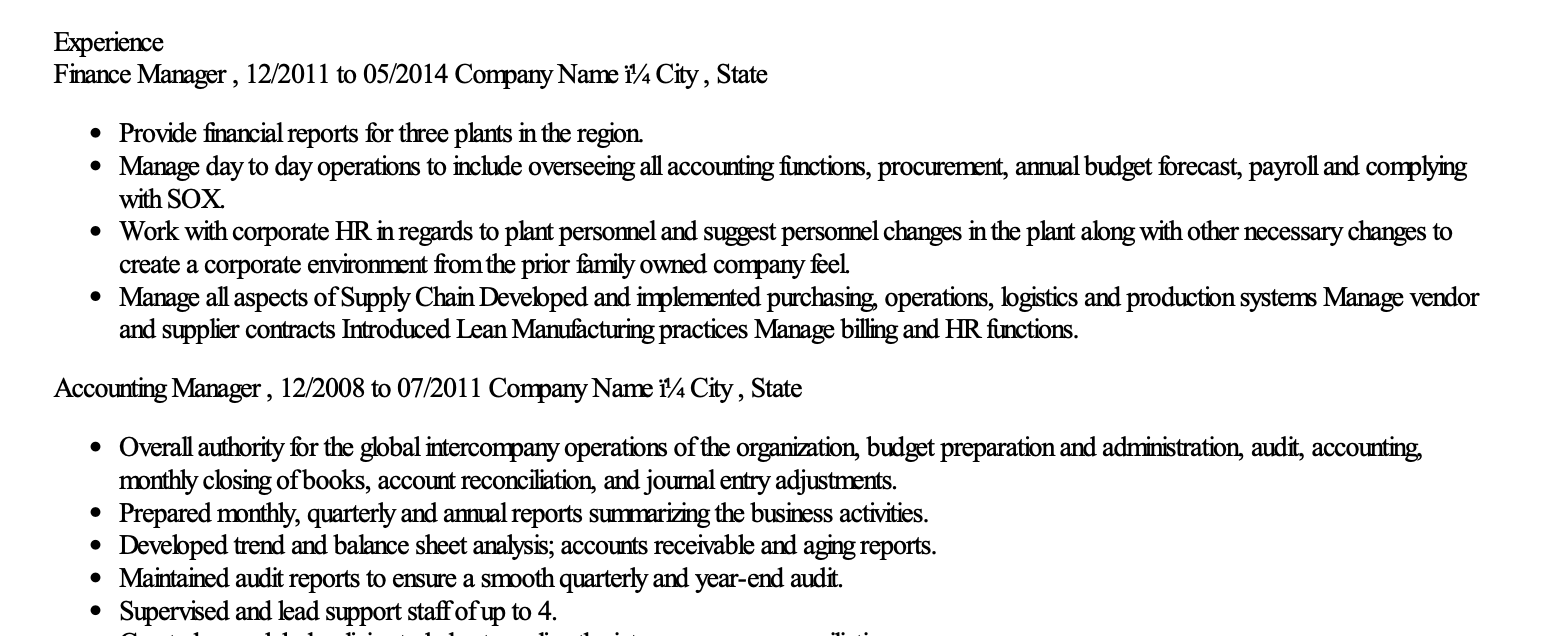
\includegraphics[width=0.5\textwidth]{cross_fields.png}}
    \caption{The resume expmale `11441764` of having cross-fields potential}
    \label{cross_fields}
\end{figure}

\begin{figure}[t]
    \centerline{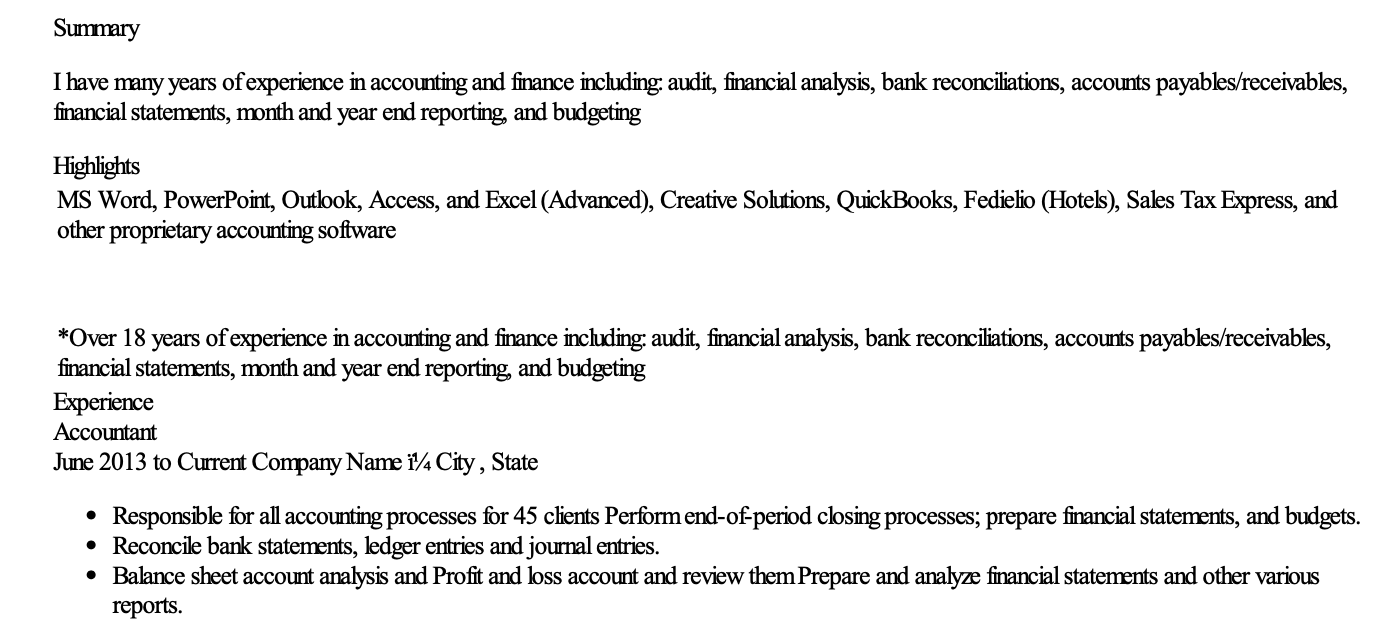
\includegraphics[width=0.5\textwidth]{resume_d_hat.png}}
    \caption{The resume $\hat{d}$ `21338490` of category `ACCOUNTTANT`}
    \label{resume_d_hat}
\end{figure}

\begin{figure}[t]
    \centerline{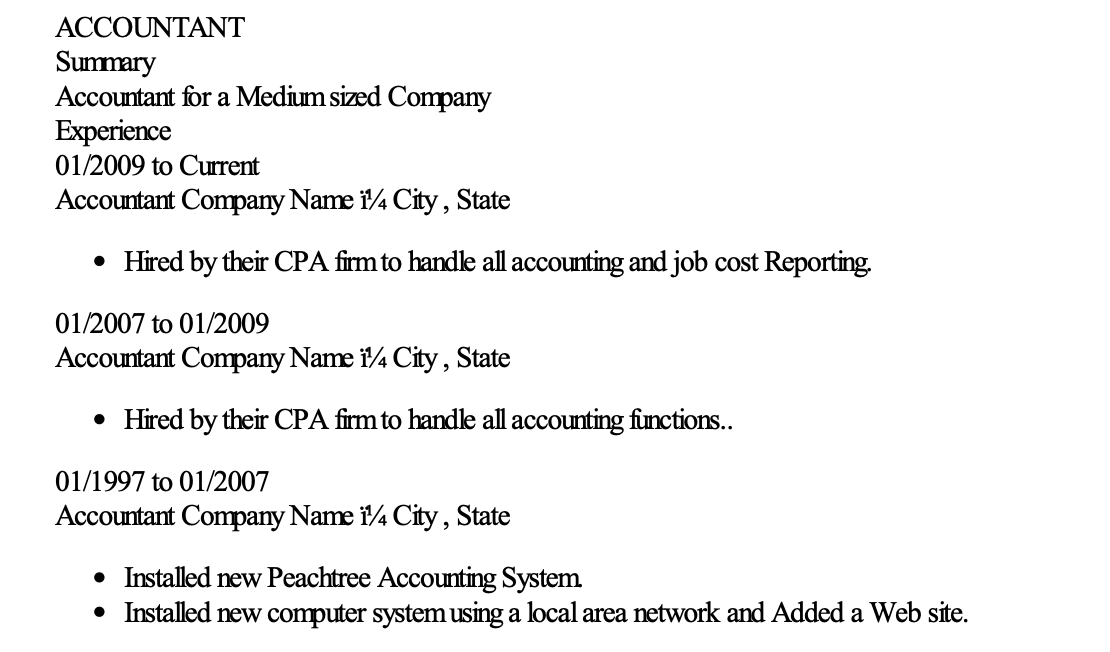
\includegraphics[width=0.5\textwidth]{resume_d_star.png}}
    \caption{The resume $d^{*}$ `24799301` of category `ACCOUNTTANT`}
    \label{resume_d_star}
\end{figure}

欲檢驗本專案提出之方法,
我們使用ACCOUNTANT、ADVOCATE及AGRICULTURE這三種求職類別進行分析作為範例,
我們找出了欲求職FINANCE之履歷,如圖.~\ref{cross_fields} 所示,
其內容可看出具有跨領域之性質,
因文字內容也有包含了ACCOUNTANT等敘述,
因此可推論我們所提出之方法具有可行性。

另一方面,
我們也針對了各職缺類別,
找出是否各有具跨領域性質之履歷,
表.~\ref{table:1}呈現本專案中所出之各類別中具有跨領域性質之履歷表,
右邊欄位`similarity`意思為$d^{*}$與$\overline{d}_{c^{'}}$之相似度,
比對各個相關性(Cosine Similarity),
該些數值皆可看出不高,
推測應為該些履歷表除了有跨領域性質外,
另一層面,
可能也代表了該些履歷表的品質不若其他同類型之履歷表高,
舉例而言,
圖.~\ref{resume_d_hat}及圖.~\ref{resume_d_star}分別代表ACCOUNTANT類別的兩種履歷($\hat{d}$,$d^{*}$),
可看出兩者的差別在於,
後者的履歷相較於前者的履歷而言,
對於ACCOUNTTANT的文字較少著墨,
因此也可推斷為該履歷相較之下較不易辨別為申請ACCOUNTANT工作。

至於跨領域性質之履歷資料,
依表.~\ref{table:1}之similariy結果而言,
似看不出顯著高之結果,
可能因為不同職缺要求之文字上的差異較大,
因此依此結果,
可能找不到適合有跨領域特性之履歷。

\section{結論}

於本專案,
我們針對了網路公開之真實履歷資料,
提出了一個簡易式之文字探勘方法,
其包含了兩個部份,
其一為檢驗該些履歷是否符合所投職缺,
其二找出是否具有跨領域性質之履歷或找出品質欠佳之履歷。

關於檢驗履歷,
我們使用了k-means作為分群方法,
在分析的過程中,
我們可看出該些履歷的分群結果數量,
與其原本求職職缺的類別數未相異過大,
再輔以資料視覺化之方法,
也可看出並無顯著之差異,
因此可推斷出此方法具有可用性。

再者,
我們提出一個簡易式之搜尋具跨領域性質之履歷資料,
而結果也可看出我們所找出之履歷資料,
的確具有跨領域之性質,
除此之外,再者我們將該些履歷資料進一步分析,
以期找出合適之具跨領域之履歷資料,
然該依結果而言,
似乎看不出有趣之履歷資料,
但也看到一些履歷在撰寫上,
不同品質上之差異,
易言之,
在履歷撰寫上,
提及跟職缺相關之文字於履歷中,
或許對履歷之品質提昇或有幫助,
因此我們也整理後附上了那些可參照之履歷(相關性高及相關性低),
以供讀者參照去查看原始履歷。

針對本專案之方法未來可延伸之議題,
也於此提出供讀者參考,
於本專案之方法結果成現,
尚缺乏深入之量化分析結果,
僅以人為判斷為主來推斷所提出之方法可用性,
另外方法是否具有泛化性(Generalization)也值得探討 \cite{murphy2012machine},
因本專案僅使用於網際網路公開之一組履歷資料,
對於該些資料之代表性,
可能也需要檢驗。

\begin{acks}
    謝謝老師上課所教授之知識,使得我們能得以完成此次報告研究。
\end{acks}

\bibliographystyle{ACM-Reference-Format}
\bibliography{mybib}

\end{document}
\endinput
